\chapter{Popis problému, specifikace cíle}
\label{chap:cile}


Jak je již předesláno v předchozí kapitole, komplexní objekty, jako je právě například vegetace, představují v oboru počítačové grafiky zvláštní kategorii s relativně vysokou složitostí jejich zpracování. Celá úloha se řádově komplikuje, požadujeme-li zobrazování v reálném čase. Problém zobrazování vegetace lze mírně abstrahovat na úlohu zobrazování stromů. S vývojem hardwaru a aplikací, které umožňují uživateli interakci s virtuálním prostředím, se zvyšují požadavky na realističnost zobrazované vegetace. Je vyžadováno nejen věrné zobrazení statického stromu, ale také jeho animace. Uvědomíme-li si však, že průměrně rostlý listnatý strom může mít až miliony jednotlivých listů a uživatel požaduje zobrazení ne jednoho stromu, ale hned celého lesa o několika tisících stromů, je přímý a naivní přístup k řešení problému příliš náročný pro současný běžný hardware. Přitom se jedná pouze o prostředí, které dotváří scénu a má významově nižší prioritu než objekty zájmu uživatele (budovy, vozidla, speciální efekty, ostatní hráči - příklady ze světa počítačových her) a tedy by jeho zpracování a zobrazování nemělo vytěžovat ve větší míře dostupné prostředky počítače.
	V následující sekci budou vytyčeny cíle této práce a definována úroveň podrobnosti, které se chce práce přiblížit. Následující text se zaměří na rešerši aktuálního stavu v oblasti real-time renderování vegetace pro vymezenou úroveň podrobnosti. V další kapitole (~\nameref{chap:analyza} ) bude rozpracován teoretický základ pro implementaci softwaru zobrazujícím vegetaci v reálném čase. Kapitola ~\nameref{chap:realizace} popíše specifika výsledné implementace a řešení postatných problémů vyplývajících z její realizace. Ověření a zhodnocení kvalit vytvořeného software se bude věnovat kapitola  ~\nameref{chap:testovani}. Poslední kapitola diskutuje výsledky práce a nastíní možné způsoby vylepšení výsledné implementace.

%%%%%%%%%%%%%%%%%%%%%%%%%%%%%%%%%%%%%%%%%%%%%%%%%%%%%%%%%%%%%%%%%%%%
\section{Vymezení cílů}
Hned na úvod je třeba vyjasnit, jaké úrovně podrobnosti (detailu) se tato práce bude snažit dosáhnout. Ačkoliv má pojem „úroveň detailu“ (Level Of Detail - LOD) v oboru CGI víceméně technický význam, je možné ho chápat i jinak, a to bez znalosti světa počítačů. V této práci jde o zobrazování rostlin – konkrétně stromů. Úrovní detailu, kterými můžeme pohlížet na stromy, je celá řada (viz obr. ~\ref{fig:Levels_of_detail}). 

\begin{figure}[!hbt]
\begin{center}
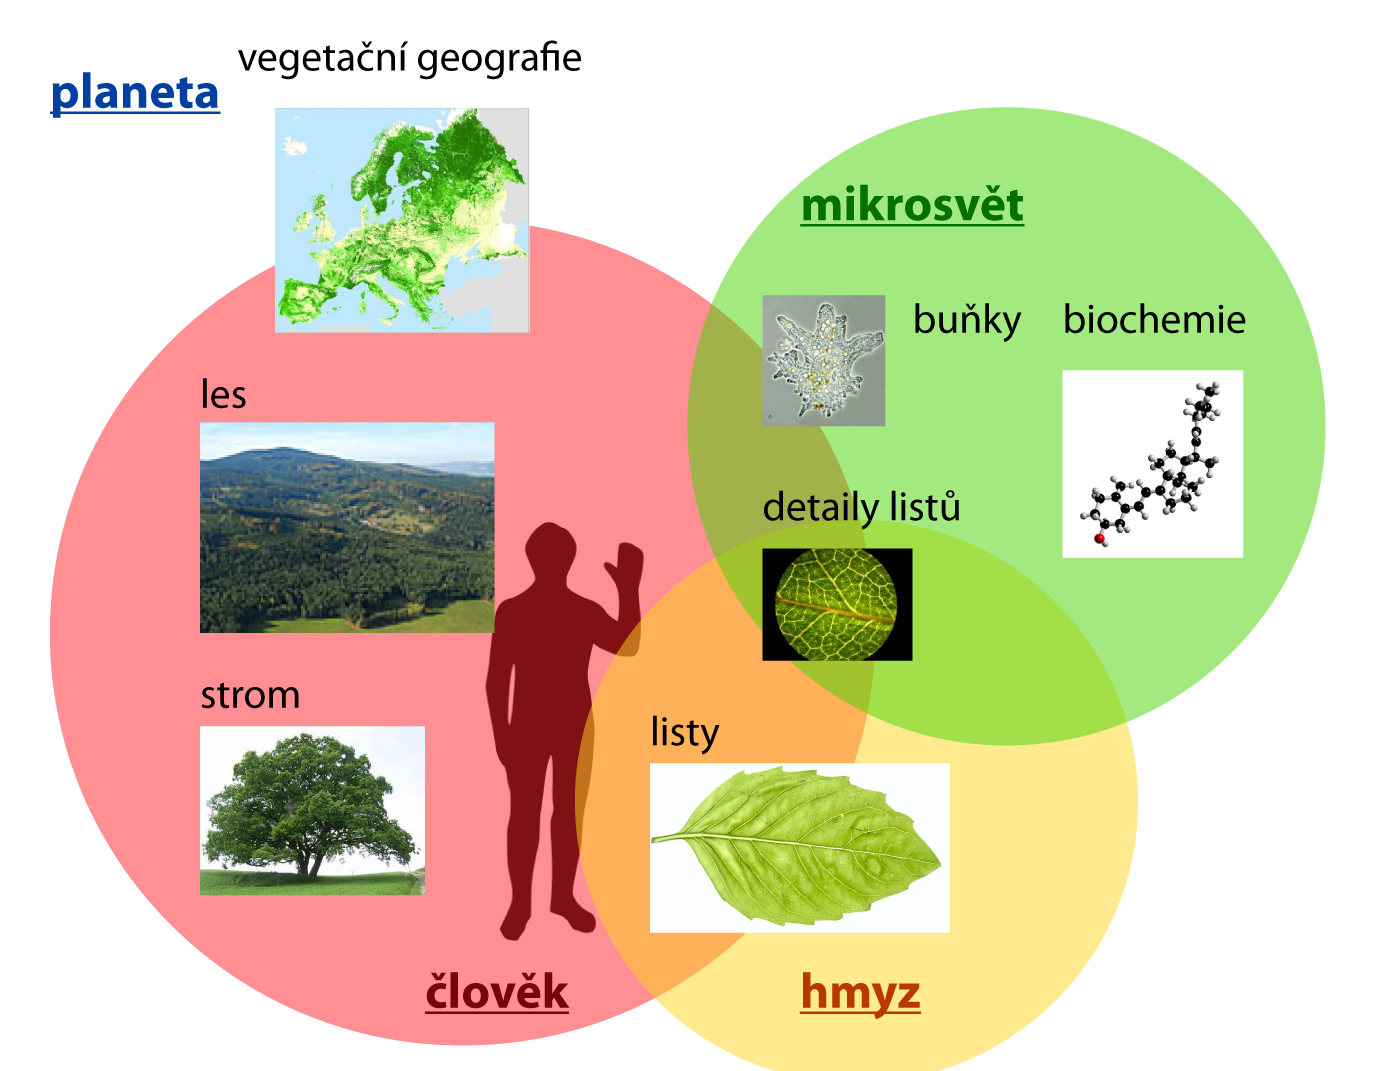
\includegraphics[width=0.7\textwidth]{./figures/DETAIL.png}

\caption{Znázornění příkladu úrovní detailu. }
\label{fig:Levels_of_detail}
\end{center}
\end{figure}

Pokud budeme na chvíli chápat úroveň detailu tímto způsobem, uveďme, že tato práce se pohybuje výhradně na úrovni pohledu člověka, neboť právě virtuální simulace pohledu člověka na vegetaci je jejím předmětem.
Samozřejmě je možné navrhnout i jiné systémy, které zpřístupní uživatelům informace na ostatních úrovních detailu, ale to je již úloha z oboru vizualizace a řada postupů by byla zřejmě zcela odlišná.
Souvislost tohoto přirozeného systému úrovní detailu s již zmíněným technickým pojetím ale existuje. Jak bude popsáno dále, v současné době není v možnostech běžného hardwaru zobrazovat jednotným postupem lesy o tisícovkách stromů i detail jednotlivých listů samostatného stromu dostatečnou rychlostí pro real-time aplikace. Přirozený systém úrovní detailu rovněž napovídá, jak uživatel vnímá určité pohledy. Při pohledu na celý rozsáhlý les stromů jsou tím nejpodrobnějším, co uživatel rozpozná, jednotlivé stromy, případně nejvýraznější větve, největší pozornost je zaměřena na celkový tvar lesa, tvar čáry horizontu, hustotu a druhovou skladbu jednotlivých rostlin. Pohled na úrovni jednotlivého stromu naproti tomu musí zobrazit i jednotlivé větve a listy, tvar lesa již není tak důležitou informací. Pokud přejdeme ještě blíž, uživatel by měl mít možnost pozorovat i detaily na listech. Z toho může vycházet technická stránka úrovně detailu (dále jen LOD).

Cílem této práce je navrhnout a realizovat software, který bude realisticky zobrazovat stromovou vegetaci v reálném čase a umožní i její animaci (působením větru). Software by měl pracovat na běžně dostupném hardware. Dále bude software poskytovat podporu pro zobrazování stromů v různých obdobích roku. Půjde především o změnu barvy listí. Práce se bude pohybovat na úrovni podrobnosti běžné pro vnímání člověka. Tedy umožní zobrazit větší skupinu stromů (les) a přitom bude možné pozorovat jednotlivé listy stromů a to včetně animace.

%%%%%%%%%%%%%%%%%%%%%%%%%%%%%%%%%%%%%%%%%%%%%%%%%%%%%%%%%%%%%%%%%%%%
\section{Stávající řešení}

Zobrazování vegetace v reálném čase je vcelku běžný požadavek současných grafických systémů - především herních enginů. Jak ukazuje například článek \cite{Mantler_2003_SARRV}, existuje množství různých přístupů. Mohou být veskrze rozděleny podle toho, zda pracují přímo s prostorovou geometrií modelu (3D reprezentace), či s dvourozměrnou náhražkou (2D reprezentace). Každý přístup má svá pro i proti a existuje i mnoho způsobů, jak je kombinovat.
 
\subsection{Trojrozměrná geometrická reprezentace}
Základní verze 3D povrchové reprezentace modelu vychází z myšlenky, že pokud je těleso neprůhledné (neprůsvitné), stačí k jeho zobrazení vykreslit jen jeho povrch. Povrch tělesa je popsán množinou trojúhelníků v prostoru a jejich barvou (texturou) - případně dalšími atributy. Trojúhelník reprezentuje část geometrie skutečného modelu. Avšak je nutné si uvědomit, že možnosti současných grafických karet jsou omezené a jejich výkon pro real-time (zhruba 25 fps) se pohybuje pouze v řádech desítek milionů zpracovaných trojúhelníků  (při základní pipeline). Tato hranice se ještě výrazně sníží, pokud požadujeme pokročilejší zpracování (například složitější model osvětlení, více texturovacích zdrojů, atd.). Z výše uvedených omezujících faktorů vyplývá, že přímé zobrazení např. celého lesa na úrovni vykreslování trojúhelníků, coby geometrie reprezentující jednotlivé listy, je příliš náročné i pro současný hardware.
Zajímavé metody a přístupy, jak zobrazovat kvalitně a efektivně i detailní geometrii stromů včetně animace až na úrovni jednotlivých listů jsou popsány v článcích \cite{Habel_09_PGT} a \cite{Habel_2007_RTT}. 
\begin{figure}[here]
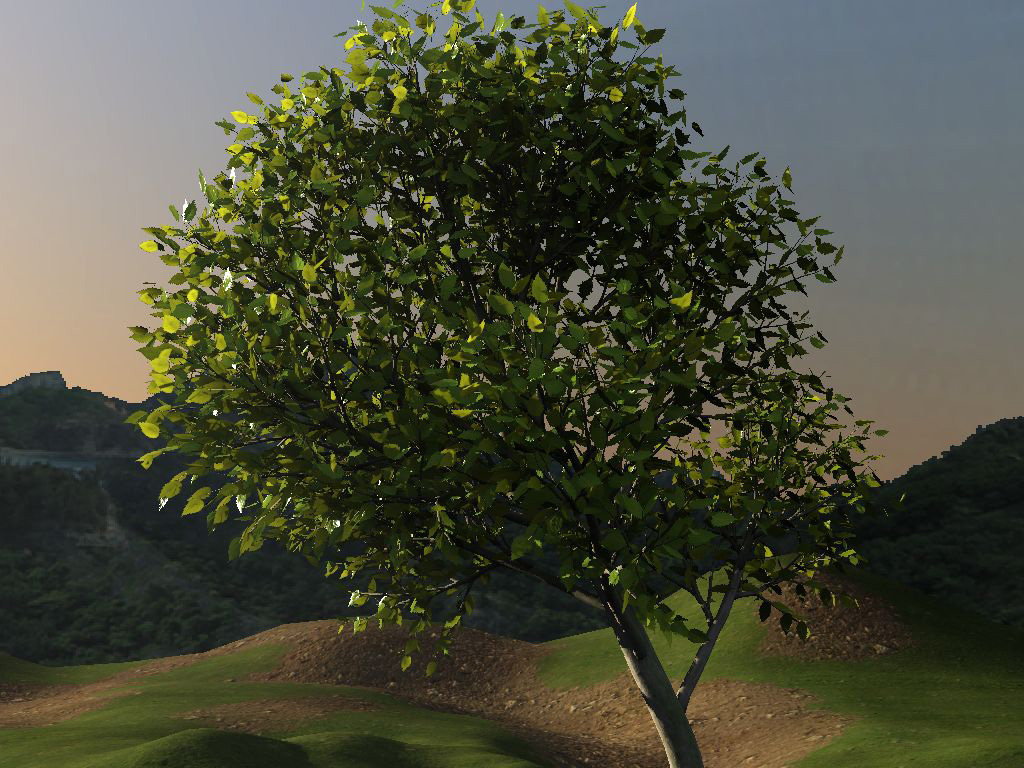
\includegraphics[width=0.5\textwidth]{./figures/HABEL_tree.jpg}
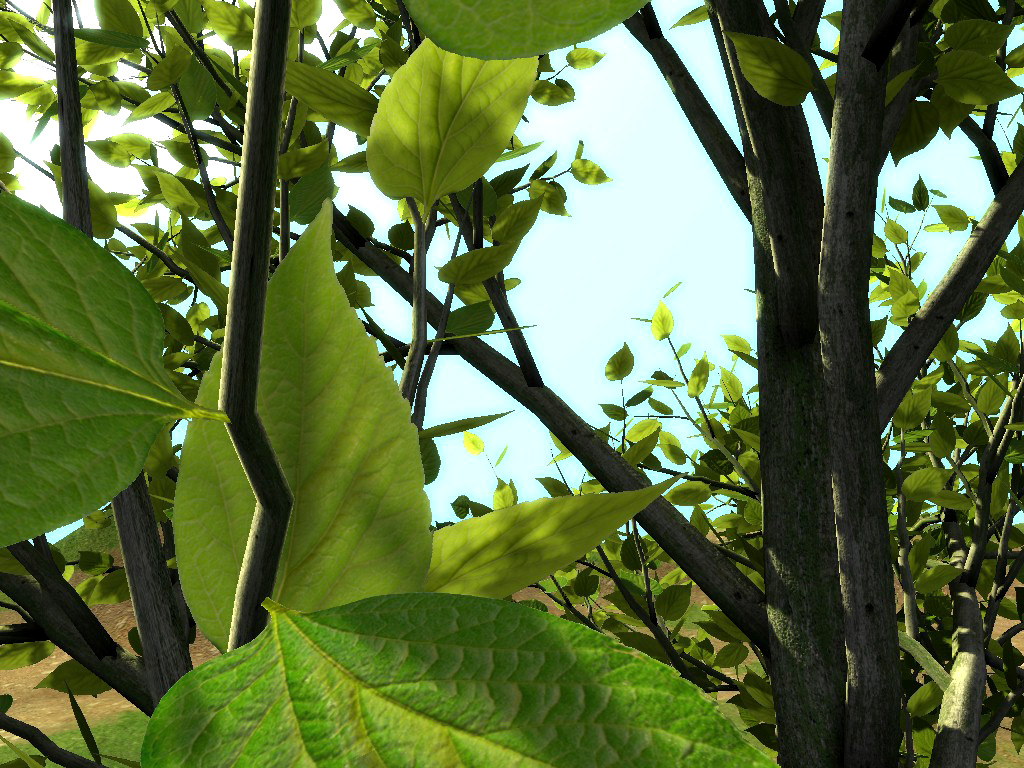
\includegraphics[width=0.5\textwidth]{./figures/HABEL_leaves.jpg}
\caption{Možnosti realistického zobrazování vegetace, převzato z \cite{Habel_2007_RTT} }
\label{fig:HABEL_leaves}
\end{figure}
Jsou navrženy postupy, které berou v potaz rozdílné vlastnosti různých stran listů i jejich průsvitnost. Animace stromu je optimalizována pro zpracování na GPU ve vertex shaderu a pracuje na principu hierarchické deformace geometrie na úrovni jednotlivých hierarchických úrovní větví. Avšak zobrazení většího počtu stromů je i tak příliš náročné na výkon a není zde řešeno.

Existuje však i možnost, jak zobrazení optimalizovat. K tomu účelu se hojně využívá technik zjednodušování geometrie 3D objektu. Složitost geometrie přechází ve složitost materiálu. Pokud zůstaneme u tématu vegetace, pak si lze představit, že původní 3D reprezentace např. stromu obsahuje geometrický popis i nejmenších detailů křivosti jednotlivých listů. V tom případě by stačila jen informace o barvě geometrických primitiv a výsledný obrázek po vykreslení by mohl být velmi kvalitní. Učiňme myšlenkový krok zjednodušení geometrie tak, že jednotlivý list reprezentuje pouze jeden trojúhelník. Křivost samotného listu pak musí obsáhnout složitější informace o materiálu listu. Pokud bychom reprezentovali např. celou větev se všemi listy jedním trojúhelníkem, složitost materiálu musí zákonitě narůst příslušným způsobem, pokud požadujeme alespoň přibližně stejný výsledek zobrazení.
%%%%%%%%%%%%%%%%%%%%%%%%%%%%%%%%%%%%%%%%%%%%%%%%%%%%%%%%%%
\pagebreak
\subsection{Reprezentace založené na obrázcích}

%\begin{figure}[here]
%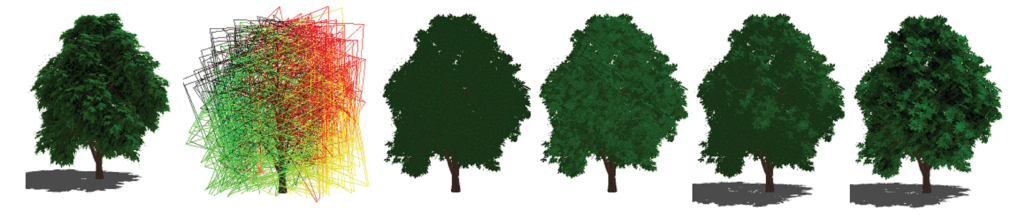
\includegraphics[width=1.0\textwidth]{./figures/garcia_billboardclouds.png}
%\caption{Reprezentace korum stromů pomocí billboadcloudů, převzato z \cite{GIPGSMSL07_images} }
%\label{fig:GARCIA_billboardcloud}
%\end{figure}


Způsob, jak optimalizovat proces zobrazování pomocí seskupení podobně orientovaných listů z celé koruny stromu do billboardů je popsán v článku \cite{GIPGSMSL07}. Vegetace je pak reprezentována tzv. billboardcloudem. Bohužel, ačkoliv je tento přístup velmi slibný pro statické modely, pokud požadujeme věrohodnou animaci vegetace, pak nelze předpokládat, že všechny obdobně orientované listy na různých větvích se budou chovat stejným způsobem.
\begin{figure}[here]
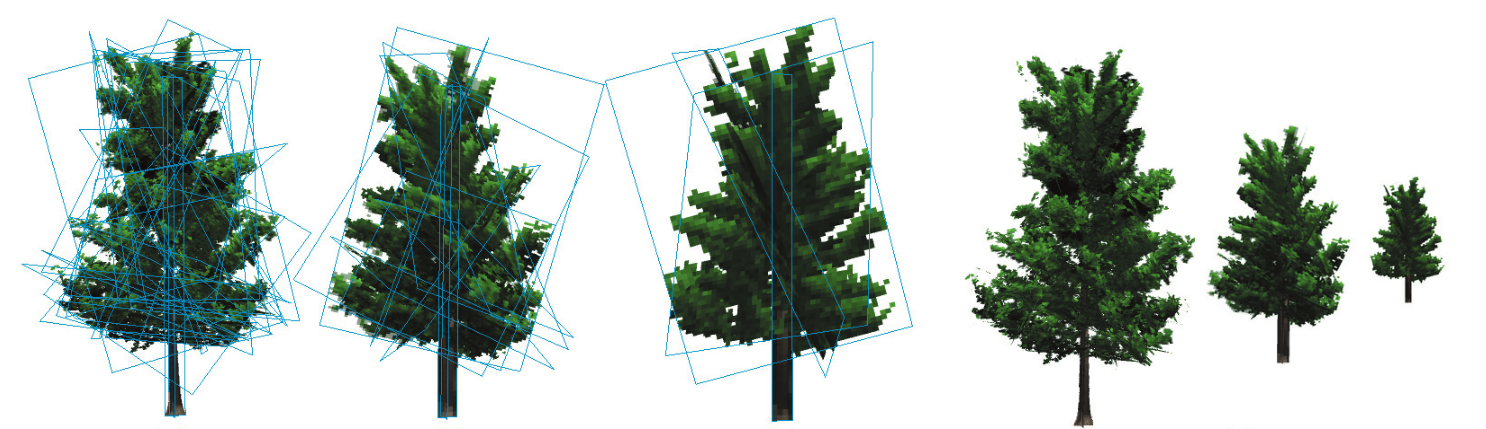
\includegraphics[width=1.0\textwidth]{./figures/umlauf_lod.png}
\caption{Různé úrovně detailu tvořené billboardy a jejich porovnání při použití (zcela vpravo), převzato z \cite{Umlauf05} }
\label{fig:UMLAUF_lod}
\end{figure}
Myšlenka seskupení blízkých listů za účelem zjednodušení geometrické složitosti modelu je vyjádřena v článku \cite{Rebollo_07_FRL}, kde jsou listy dynamicky slučovány na základě jejich prostorové blízkosti a podobnosti. Ačkoliv jsou navrhované postupy daleko vhodnější pro přidání možnosti animace, jde v zásadě o dynamické řízení úrovně detailu a jako takové vyžadují relativně výrazné prostředky pro správu zjednodušovaného modelu. 

Existuje i několik přístupů založených čistě na billboardingu. Metoda řezů představená v článku \cite{Jakulin00} vytváří určitý trs billboardů, které zobrazují pohledy z několika směrů a to i v několika vrstvách (viz obr. ~\ref{fig:JAKULIN_slices}).
\begin{figure}[!htb]
\begin{center}
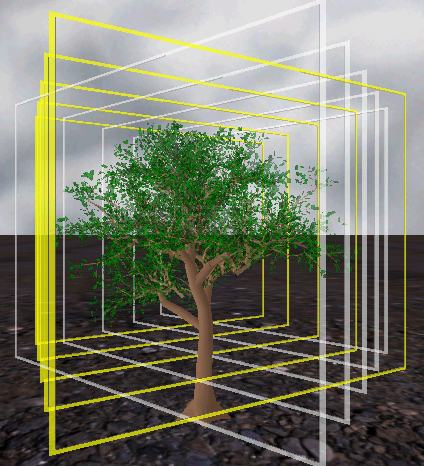
\includegraphics[width=0.3\textwidth]{./figures/slicingJakulin.jpg}
\end{center}
\caption{Reprezentace korum stromů pomocí řezů, převzato z \cite{Jakulin00} }
\label{fig:JAKULIN_slices}
\end{figure}
 Trs billboardů je v tomto případě vůči scéně nehybný a řezy, které jsou souběžné se směrem pohledu, jsou skrývány. Výhoda použití více souběžných billboardů spočívá v tom, že lze tímto způsobem navodit dojem určité prostorové hloubky (efekt paralaxy).

Metoda trsu rovnoběžných billboardů je rozpracována i v článku \cite{Truelsen_08}, kde je popsána možnost, jak efektivně řídit úrovně detailu pro tyto trsy.

Dovedeme-li zjednodušení do takové krajnosti, že původní objekt (či dokonce skupiny objektů) reprezentujeme jedním geometrickým primitivem, mluvíme o takzvaných billboardech, či impostorech (viz obr. ~\ref{fig:UMLAUF_billboards}). 
Díky vlastnostem lidského vnímání a zobrazovací technoliogii je možné nahradit určitý objekt plochým obrazem, který odpovídá pohledu na daný objekt z podobného místa. 
\begin{figure}[!htb]
\begin{center}$
\begin{array}{cc}
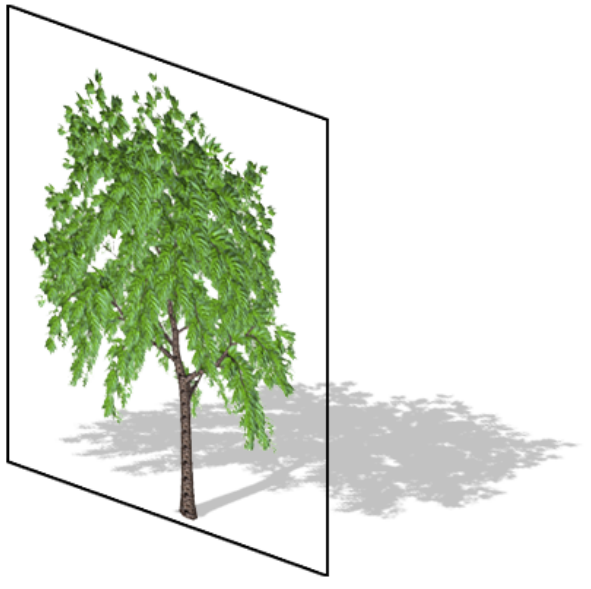
\includegraphics[width=0.25\textwidth]{./figures/billboard_a.png}&
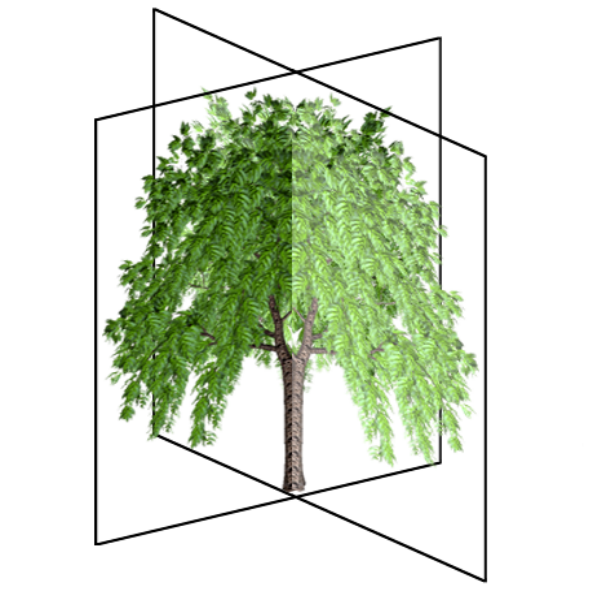
\includegraphics[width=0.25\textwidth]{./figures/billboard_b.png}\\
(a)&(b)
\end{array}$
\end{center}
\caption{Různé přístupy k billboardům. Jediný plochý obraz, který se natáčí k pozorovateli $(a)$ , křížová konstrukce dvou billboardů, které zachovávají orientaci vůči scéně $(b)$, převzato z \cite{Umplauf_MT} }
\label{fig:UMLAUF_billboards}
\end{figure}
Zatímco zpracování geometrických primitiv je relativně pomalý proces, uplatnění informací o materiálu v daném bodě může být velmi efektivní. Nutno ovšem dodat, že běžné reprezentace materiálu (obrázkové textury) trpí omezeními plynoucími z jejich principu – např. omezené rozlišení. Tedy jakési plnohodnotné nahrazení původní 3D geometrie funguje obstojně jen pro objekty ležící za určitou rozlišovací hranicí, která je dána zejména faktory jako rozlišení textur, rozlišení obrazovky, detailnost pohledu, geometrická podobnost obou reprezentací a podobně. 

\begin{figure}[!htb]
\begin{center}
$\begin{array}{ccc}
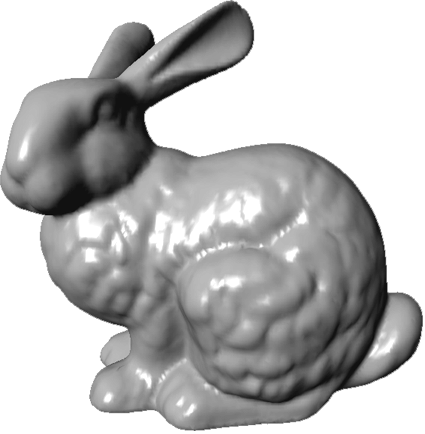
\includegraphics[width=0.2\textwidth]{./figures/bunny_lod_0.png}&
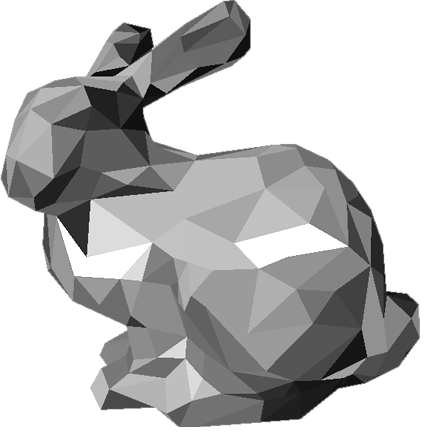
\includegraphics[width=0.2\textwidth]{./figures/bunny_lod_3.png}&
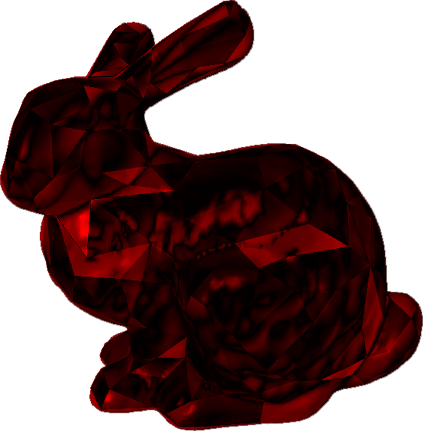
\includegraphics[width=0.2\textwidth]{./figures/bunny_lod_diff.png}
\\
(a)&(b)&(c)
\end{array}$
\end{center}
\caption{Obrazy různých stupňů detailu téhož modelu $(a)$ a $(b)$ a jejich rozdíl červeně $(c)$}
\label{fig:BUNNY_lod}
\end{figure}
Pokud metoda zobrazování a řízení úrovně detailu nepracuje dynamicky (což většinou zajišťuje takřka nepostřehnutelný přechod mezi úrovněmi), vyvstává vždy problém, jak provádět přechod mezi jednotlivými úrovněmi, který při naivním přepnutí úrovní může vést k nevítanému efektu zvanému \emph{LOD-popping}. Jde o to, že pokud se skokově změní velká část obrazu, vnímá tuto změnu pozorovatel velmi rušivě.
Klasická metoda snížení LOD-poppingu pracuje s prolínáním obrazů a řízením jejich průhlednosti. Zatímco jedna úroveň je postupně zprůhledňována a mizí, druhá se naopak stává neprůhlednou a objevuje se. Během tohoto přechodu se ovšem může stát, že se model stane průhledným, jak ukazuje obrázek  ~\ref{fig:BUNNY_lod_trans}.
\begin{figure}[!htb]
\begin{center}
$\begin{array}{ccc}
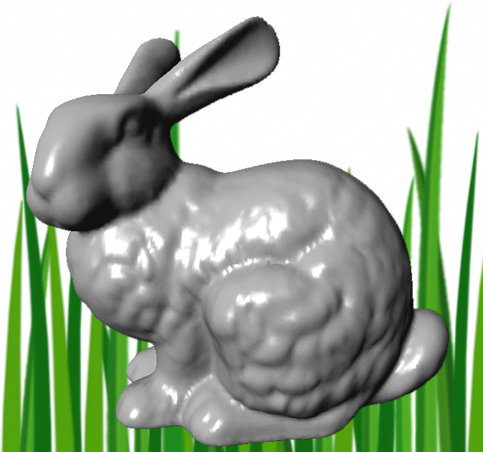
\includegraphics[width=0.2\textwidth]{./figures/bunny_lod_trans_01.png}&
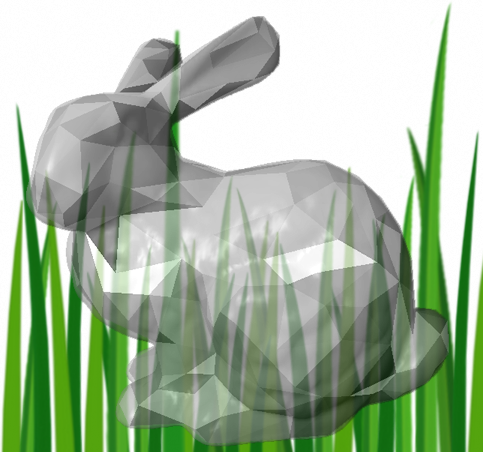
\includegraphics[width=0.2\textwidth]{./figures/bunny_lod_trans_02.png}&
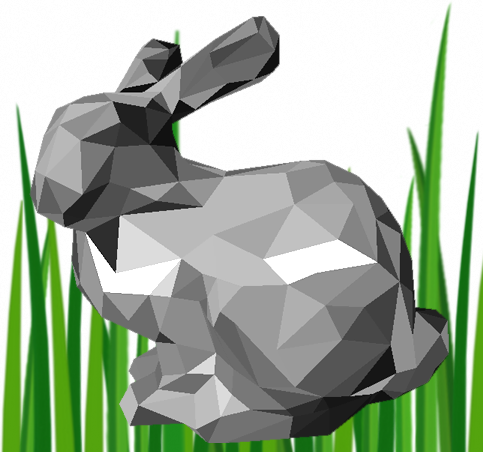
\includegraphics[width=0.2\textwidth]{./figures/bunny_lod_trans_03.png}
\\
(a)&(b)&(c)
\end{array}$
\end{center}
\caption{Znázornění problémů měkkého přechodu mezi diskrétními úrovněmi detailu.
\newline
$(a)$ LOD0 100\% , LOD1 0\% \newline
$(b)$ LOD0 50\% , LOD1 50\%, objekt se stal průhledným, ačkoliv by neměl. \newline
$(c)$ LOD0 0\% , LOD1 100\% 
}
\label{fig:BUNNY_lod_trans}
\end{figure}
Eliminací tohoto nežádoucího efektu se zabývá článek \cite{GIEGL-2007-UNP}. Jde o postup, kdy je vždy jedna úroveň detailu zobrazena plně a neprůhledně. Tím je zaručeno, že nemůže dojít k celkovému zprůhlednění. 

%%%%%%%%%%%%%%%%%%%%%%%%%%%%%%%%%%%%%%%%%%%%%%%%%%%%%%%%%%
\subsection{Volumetrické renderování a pointcloudy}
Existují však ještě další možnosti, jak reprezentovat a zobrazovat vegetaci. Metoda vycházející z principů volumetrického renderování (a 3D textur) je popsána v článku \cite{DN04}. Je vhodná zejména pro úroveň detailu typu les a vegetační geografie. Nicméně její přímé využití pro zobrazování na úrovni jednotlivých listů je s dnešním běžným hardware nemožné. Metoda pracuje s rovnoběžnými vrstvami textur, jejichž hustota je řízena aktuální úrovní detailu v daném místě.
\begin{figure}[here]
\begin{center}
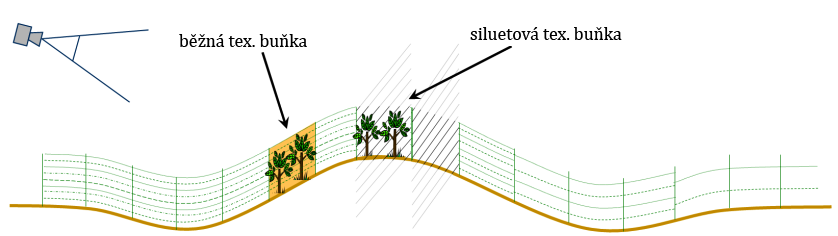
\includegraphics[width=1.0\textwidth]{./figures/a1_slicing.png}
\end{center}
\caption{Volumetrické renderování využívající rovnoběžných textur, převzato z \cite{DN04}
}
\label{fig:VOLUME_texcells}
\end{figure}

Další možností je tzv. \emph{point-based} renderování. Základním primitivem tohoto přístupu zobrazování je prostorový bod (dále jen bod). Tato metoda je výhodná zejména pro objekty, které jsou promítnuty do malého počtu pixelů na výstupním zařízení, neboť pro jejich věrné zobrazení stačí minimálně tolik bodů, kolik pixelů na zobrazovacím zařízení zabírají. Ovšem neplatí zde, že prostorový bod je vždy promítnut do právě jednoho pixelu. Velikost a tvar, jímž je reprezentován bod, se mohou lišit. Nabízí se tedy, aby list stromu byl reprezentován právě jedním bodem. Ovšem i tehdy by byl počet zpracovávaných bodů příliš veliký při zobrazování celého lesa naivním postupem. Pokročilé techniky LOD jsou navrženy v článku \cite{GMN05}. Prostor je rozdělen do pravidelné mřížky a v rámci vzniklých buněk je určen LOD. Na nejvyšší úrovni LOD reprezentuje skutečně každý bod specifický list, ovšem s nižší úrovní LOD jsou listy slučovány a postupně reprezentovány většími body (viz obr. ~\ref{fig:PB}) . 
\begin{figure}[!hbt]
\begin{center}
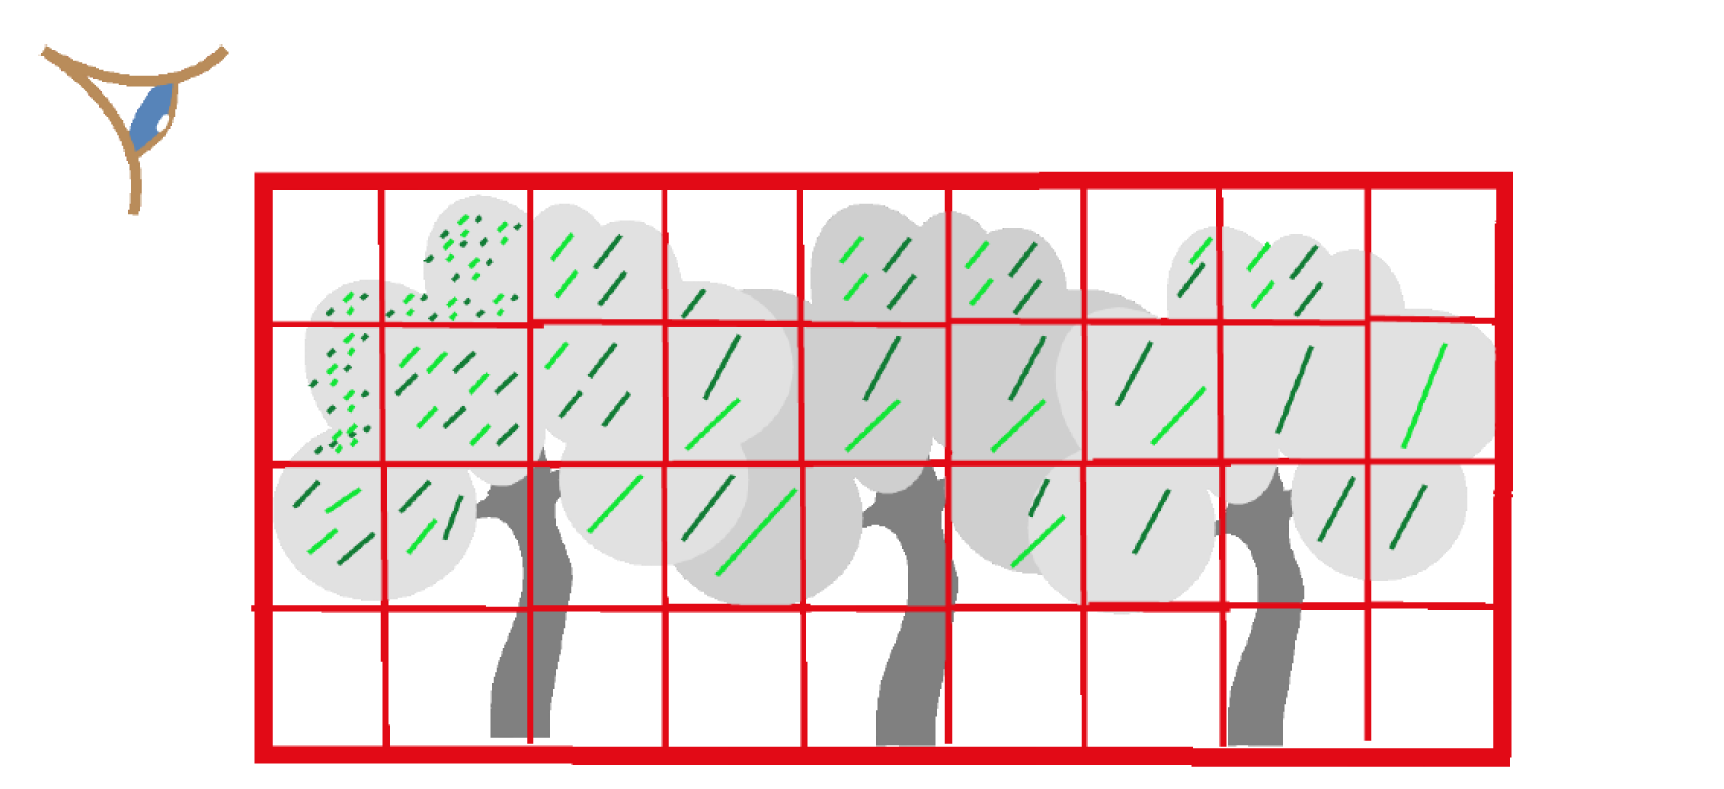
\includegraphics[width=1.0\textwidth]{./figures/point-based.png}
\end{center}
\caption{Reprezentace listů jednotlivými body. Čím je zobrazovaný bod dále od kamery, tím je větší a reprezentuje více listů. Převzato z \cite{GMN05}
}
\label{fig:PB}
\end{figure}
 
Vzdálenější koruny stromů jsou tak reprezentovány malým počtem velkých bodových primitiv, protože platí předpoklad, že tyto primitiva se zobrazí do jednoho (maximálně několika málo) výsledných pixelů. Bodová reprezentace v tomto podání funguje velmi dobře jen pro korunu stromu. Použití i pro samotný kmen a větve stromu je problematické. 
%%%%%%%%%%%%%%%%%%%%%%%%%%%%%%%%%%%%%%%%%%%%%%%%%%%%%%%%%%
\pagebreak
\subsection{Zhodnocení stávajících řešení}
Jak se ukazuje, všechna řešení pracující až na úrovni jednotlivých listů pracují s geometrickým trojrozměrným modelem stromu (povrchová trojúhelníková reprezentace). Každá z metod zobrazující současně strom na úrovni listů i rozsáhlý les využívá nějakou formu řízení úrovně detailu. Tím dosahují snížení složitosti scény a vyšší efektivity. Zatímco metod zaměřujících se pouze na statické zobrazení je celá řada, postupů, jak jednotlivé stromy realisticky rozhýbat je málo a omezují se na geometrické modely. Některé techniky LOD by bylo obtížné přizpůsobit, aby efektivně fungovaly i pro pohybující se stromy (volumetrické reprezentace). Jiné by bylo možné s relativně rozumným úsilím rozšířit i o tuto možnost (billboard-clouds). Metody dynamického řízení úrovně detailu většinou představují elegantní řešení, které netrpí problémy LOD-poppingu, ale vyžaduje zvýšené prostředky na neustálé udržování aktuální úrovně detailu modelů. Naproti tomu diskrétní LOD systémy se musí vypořádávat s přepínáním jednotlivých úrovní, ale představují jen malou výkonostní zátěž. Ať už dynamické či diskrétní LOD systémy, nejčastěji se využívá převedení složitosti geometrie do obrazu, který je pak namapován na zjednodušenou geometrii.

